\section*{Anhang}
Link zur Webanwendung:\\\url{http://www-stud.uni-due.de/~simibark/visualisierung-platonische-koerper/}
\subsection*{Bemerkung zur Webanwendung}
Die Webanwendung „Visualisierung der Platonischen Körper“ wurde mit Java Script In Linux Google Chrome 38 entwickelt. Die Benutzeroberfläche der Visualisierung wurde mit dem Open Source Projekt „Polymer“ (\url{www.polymer-project.org}), welches der BSD Lizenz unterliegt, realisiert. Für die 3D Simulation wurde auf ThreeJS (\url{www.threejs.org}) zurückgegriffen, welches der MIT Lizenz unterliegt.\\
Zuverlässig getestet wurde die Visualisierung mit IE 11 unter Windows 7, mit Safari 8 unter Mac OS X 10.10 und Google Chrome 38 unter Linux, Windows 7 und Mac OS X 10.10. Für mobile Endgeräte wurde die Anwendung im Browser Google Chrome für Android und Firefox Mobile für Android getestet.
\subsection*{Anleitung zur Webanwendung}
\begin{figure}[H]
    \centering
        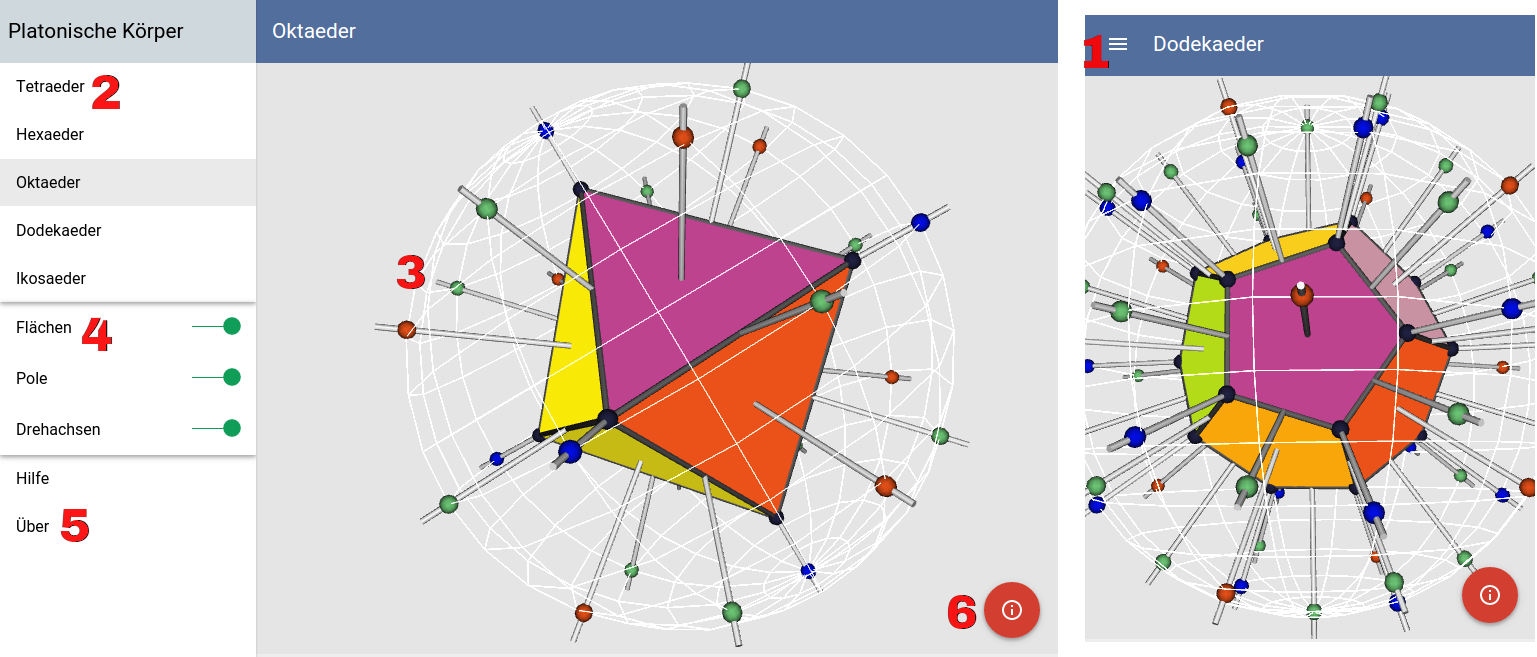
\includegraphics[width=0.95\linewidth]{grafiken/anwendung.png}

\end{figure}
\begin{enumerate}
    \setlength{\itemsep}{-4pt}
    \item Menü-Icon: öffnet das Menü mit weiteren Optionen
    \item Liste der Polyeder: mit einem Klick wird das gewünschte Polyeder angezeigt
    \item Das ausgewählte Polyeder kann durch Scrollen vergrößert bzw. verkleinert sowie durch Ziehen der Maus gedreht werden.
    \item Mit dem Umschalter können Flächen, Pole und Drehachsen ein- bzw. ausgeblendet werden. Die drei Umschalter sind unabhängig voneinander beliebig kombinierbar.
    \item Menüpunkt „Über“: enthält allgemeine Bemerkungen zur Anwendung
    \item Info-Button: mit einem Klick werden Informationen zu den Körpern geliefert: insbesondere zur Gestalt, zur Drehgruppe sowie zu den Polen.
\end{enumerate}
